\documentclass[11pt,french]{article} % police taille 11 car 10 c'est pour les terroristes
\usepackage{babel} % paquet qui permet de gérer les différentes langues
\usepackage{graphicx} % paquet pour inclure des images
\usepackage{float}
\usepackage{titling}
\usepackage{geometry}
\geometry{legalpaper, margin=100pt}

\begin{document}

\begin{figure}[t]
    \centering
		\advance\leftskip-0.2cm
    
\includegraphics[width=8cm]{inp_n7.png} % joli logo de l'N7
\end{figure}

\title{\vspace{0.5cm} \textbf{Rapport de bureau d'études\\Automatique Systèmes Cyber Physique}} 
\author{RAGOT Cyrian}
\renewcommand{\maketitlehookc}{%
	\vspace{3cm}
  \begin{center}
		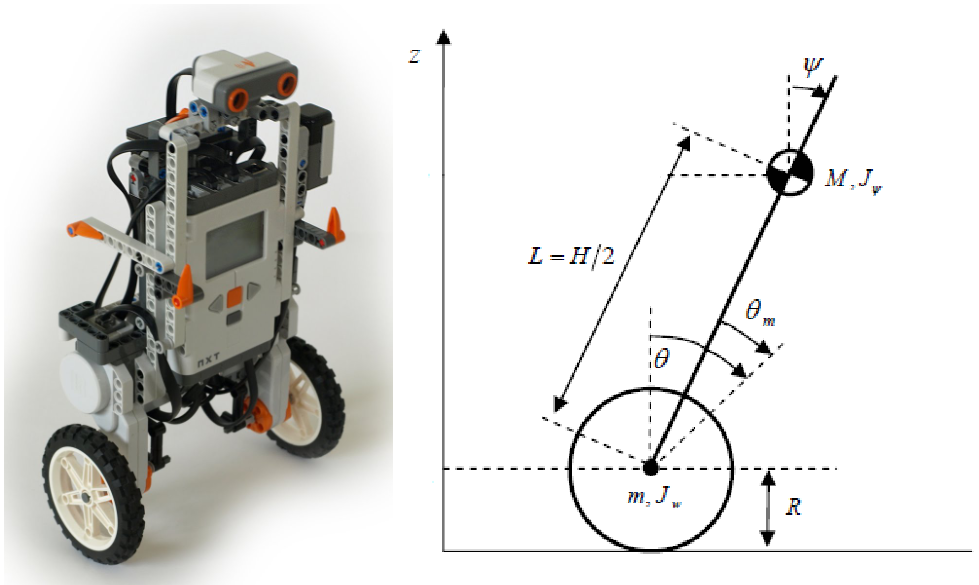
\includegraphics[width=14cm]{segway.png}
  \end{center}
}
\date{\vspace{1cm}\vfill Département Sciences du Numérique - Première année \\
2023-2024 }

\maketitle

\newpage % génère un saut de page, en gros retour à la ligne mais pour une page
\tableofcontents % génère un sommaire des sections du document
\newpage

\section{Introduction}


\newpage
\section{Modèle du pendule inversé}

\newpage
\section{Modèle du robot Lego}

\newpage
\section{Robot Lego NXT}

\newpage
\section{Conclusion}


\end{document}
